% -------
% THEORIE
% -------

% Defining TOC's sections before content
\section{Théorie}

\subsection{Modèle d'impureté d'Anderson}

\subsection{Formalisme de Green}

\begin{frame}
    \vfill
    \begin{center}
        \large
        Théorie
    \end{center}
    \vfill
\end{frame}

\begin{frame}
    \frametitle{Théorie - Modèle d'impureté d'Anderson}
    Hamiltonien du modèle d'impureté d'Anderson\footnotemark:
    \begin{align}
        \vb{H}_{\text{AIM}} &= \sum_{i,j,\sigma}t_{ij}c_{i,\sigma}^\dagger c_{j,\sigma} + U\sum_in_{i\uparrow}n_{i\downarrow} - \mu\sum_{i,\sigma}n_{i,\sigma} + \nonumber\\
            &\hspace{0.45cm}\sum_{i,\nu,\sigma}(\theta_{i\nu,\sigma}c_{i,\sigma}^\dagger a_{\nu,\sigma} + \text{h.c.}) + \sum_{\nu,\sigma}\epsilon_{\nu,\sigma}a^\dagger_{\nu,\sigma}a_{\nu,\sigma},
        \label{eq: H_AIM}
    \end{align}
    \pause
    \begin{defblock}{Définition: Opérateurs d'échelle}
        Les opérateurs $c^\dagger, c$ sont des opérateurs de création/annihilation dans la base des
        sites. $a^\dagger, a$ jouent le même rôle pour les sites de bain.
    \end{defblock}
    \footnotetext{Maxime Charlebois. "Théorie de champ moyen dynamique pour les
    système inhomogènes". \textcolor{hard_green}{Thèse de doct. Université Laval 2015}.}
\end{frame}

\begin{frame}
    \frametitle{Théorie - Modèle d'impureté d'Anderson}
    \begin{columns}
        \column{0.5\linewidth}
        Termes de Hubbard:
        {\scriptsize
        \begin{align*}
            \vb{H}_{\text{AIM}} &= \sum_{i,j,\sigma}t_{ij}c_{i,\sigma}^\dagger c_{j,\sigma} + U\sum_in_{i\uparrow}n_{i\downarrow} \\
                                &- \mu\sum_{i,\sigma}n_{i,\sigma} + \dots
        \end{align*}
        }
        \column{0.5\linewidth}
        \begin{figure}
           \centering
            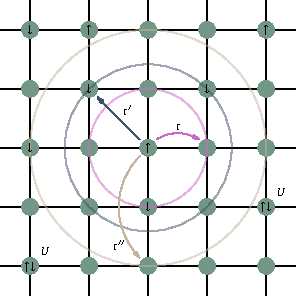
\includegraphics[scale=0.95]{./figures/theory/2d_lattice.pdf}
            % \caption{Schéma du modèle de Hubbard pour un réseau cristallin en 2 dimensions.}
            \label{fig: hubbard_2d}
        \end{figure}
    \end{columns}
\end{frame}

\begin{frame}
    \frametitle{Théorie - Modèle d'impureté d'Anderson}
    \begin{columns}
        \column{0.55\linewidth}
        Termes liés à l'impureté:
        {\scriptsize
        \begin{align*}
            \vb{H}_{\text{AIM}} &= \dots + \sum_{i,\nu,\sigma}(\theta_{i\nu,\sigma}c_{i,\sigma}^\dagger a_{\nu,\sigma} + \text{h.c.}) \\
                                &\hspace{0.8cm}+\sum_{\nu,\sigma}\epsilon_{\nu,\sigma}a^\dagger_{\nu,\sigma}a_{\nu,\sigma}
        \end{align*}
        }
        \column{0.45\linewidth}
        \begin{figure}
           \centering
            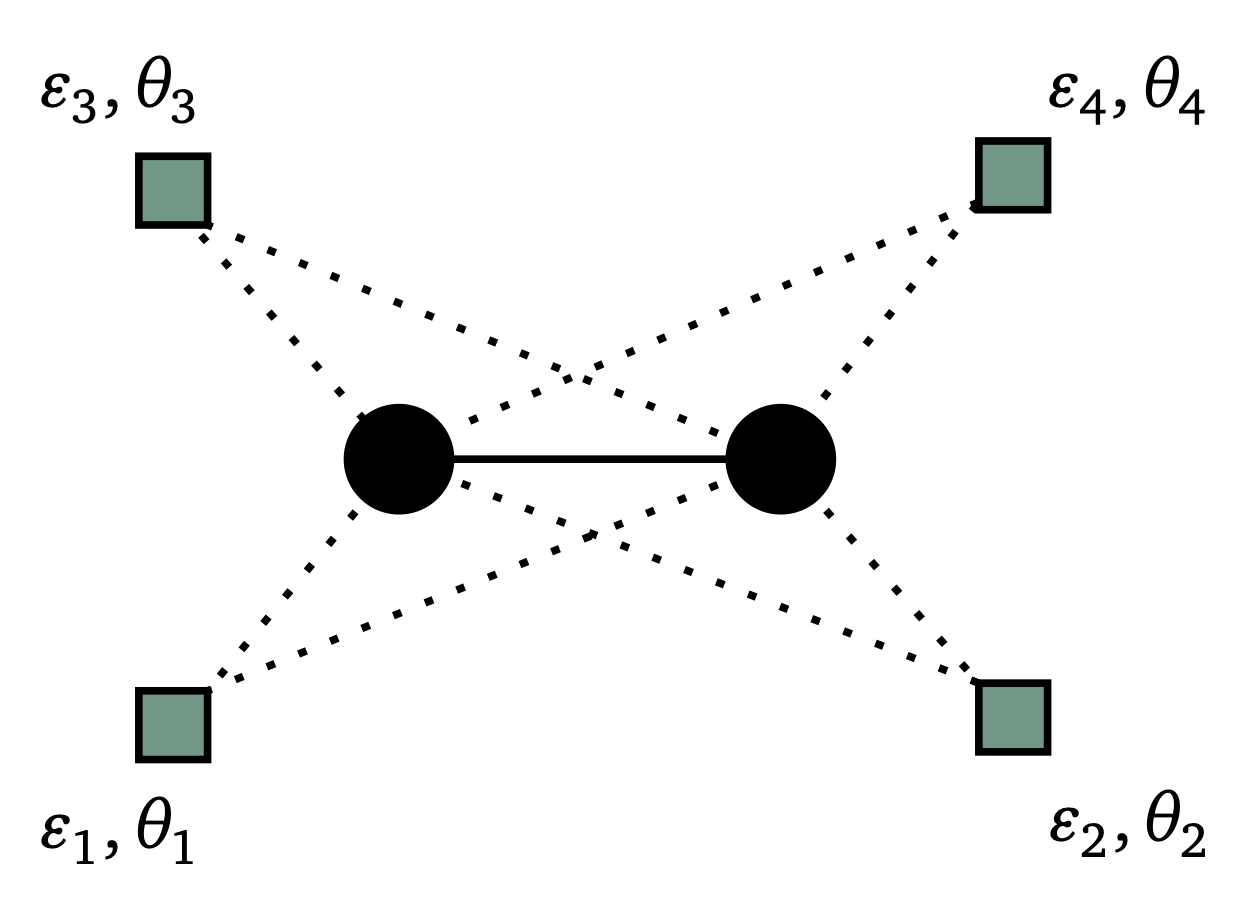
\includegraphics[scale=0.2]{./figures/theory/1D_2s_4b_cluster.png}
            % \caption{Schéma d'un amas de deux sites réels liés à 4 sites de bain.}
            \label{fig: 1D_2s_4b_HAIM}
        \end{figure}
    \end{columns}
\end{frame}

\begin{frame}
    \frametitle{Théorie - Formalisme de Green}
    L'accès aux observables se fait via la fonction de Green retardée\footnotemark
    \begin{align}
        G_{\mu\nu}(t) = -i\Theta(t)\langle c_\mu(t)c_\nu^\dagger + c_\nu^\dagger c_\mu(t)\rangle.
        \label{eq: green_retarded}
    \end{align}
    \vspace{1cm}
    \pause
    \begin{noteblock}{Note: Dépendance temporelle}
      La dépendance de $G_{\mu\nu}(t)$ au hamiltonien $\vb{H}$ est dissimulée dans la définition de l'opérateur $c_\mu(t) = e^{i\vb{H}t}c_\mu e^{-i\vb{H}t}$.
    \end{noteblock}
    \footnotetext{Maxime Charlebois. "Théorie de champ moyen dynamique pour les
    système inhomogènes". \textcolor{hard_green}{Thèse de doct. Université Laval 2015}.}
\end{frame}

\begin{frame}
    \frametitle{Théorie - Formalisme de Green}
    Équations matricielles obtenues grâce aux éqs. du mouvement $\dot{G}_{\mu\nu}(t)$
    \begin{align}
      \underbrace{\vb{G}_0^{-1} = z - \vb{t},}_{\text{sans interactions}}
        &&\underbrace{\vb{G}^{-1} = \vb{G}_0^{-1} - \vb{\Sigma}}_{\text{avec interactions}}
        \label{eq: greens}
    \end{align}
    \vfill
    \pause
    \begin{defblock}{Définition: \textit{self-énergie} $\vb{\Sigma}$}
      La \textit{self-énergie} est une quantité dont nous avons peu d'information.
      On peut la voir comme l'effet de l'interaction sur la propagation d'un électron
      (ex: piscine à balles).
    \end{defblock}
\end{frame}

\begin{frame}
    \frametitle{Théorie - Formalisme de Green}
    La nature de la CDMFT nous encourage a utiliser la base mixte ici
    représentée\footnotemark pour exprimer les fonctions de Green
    \begin{figure}
      \centering
      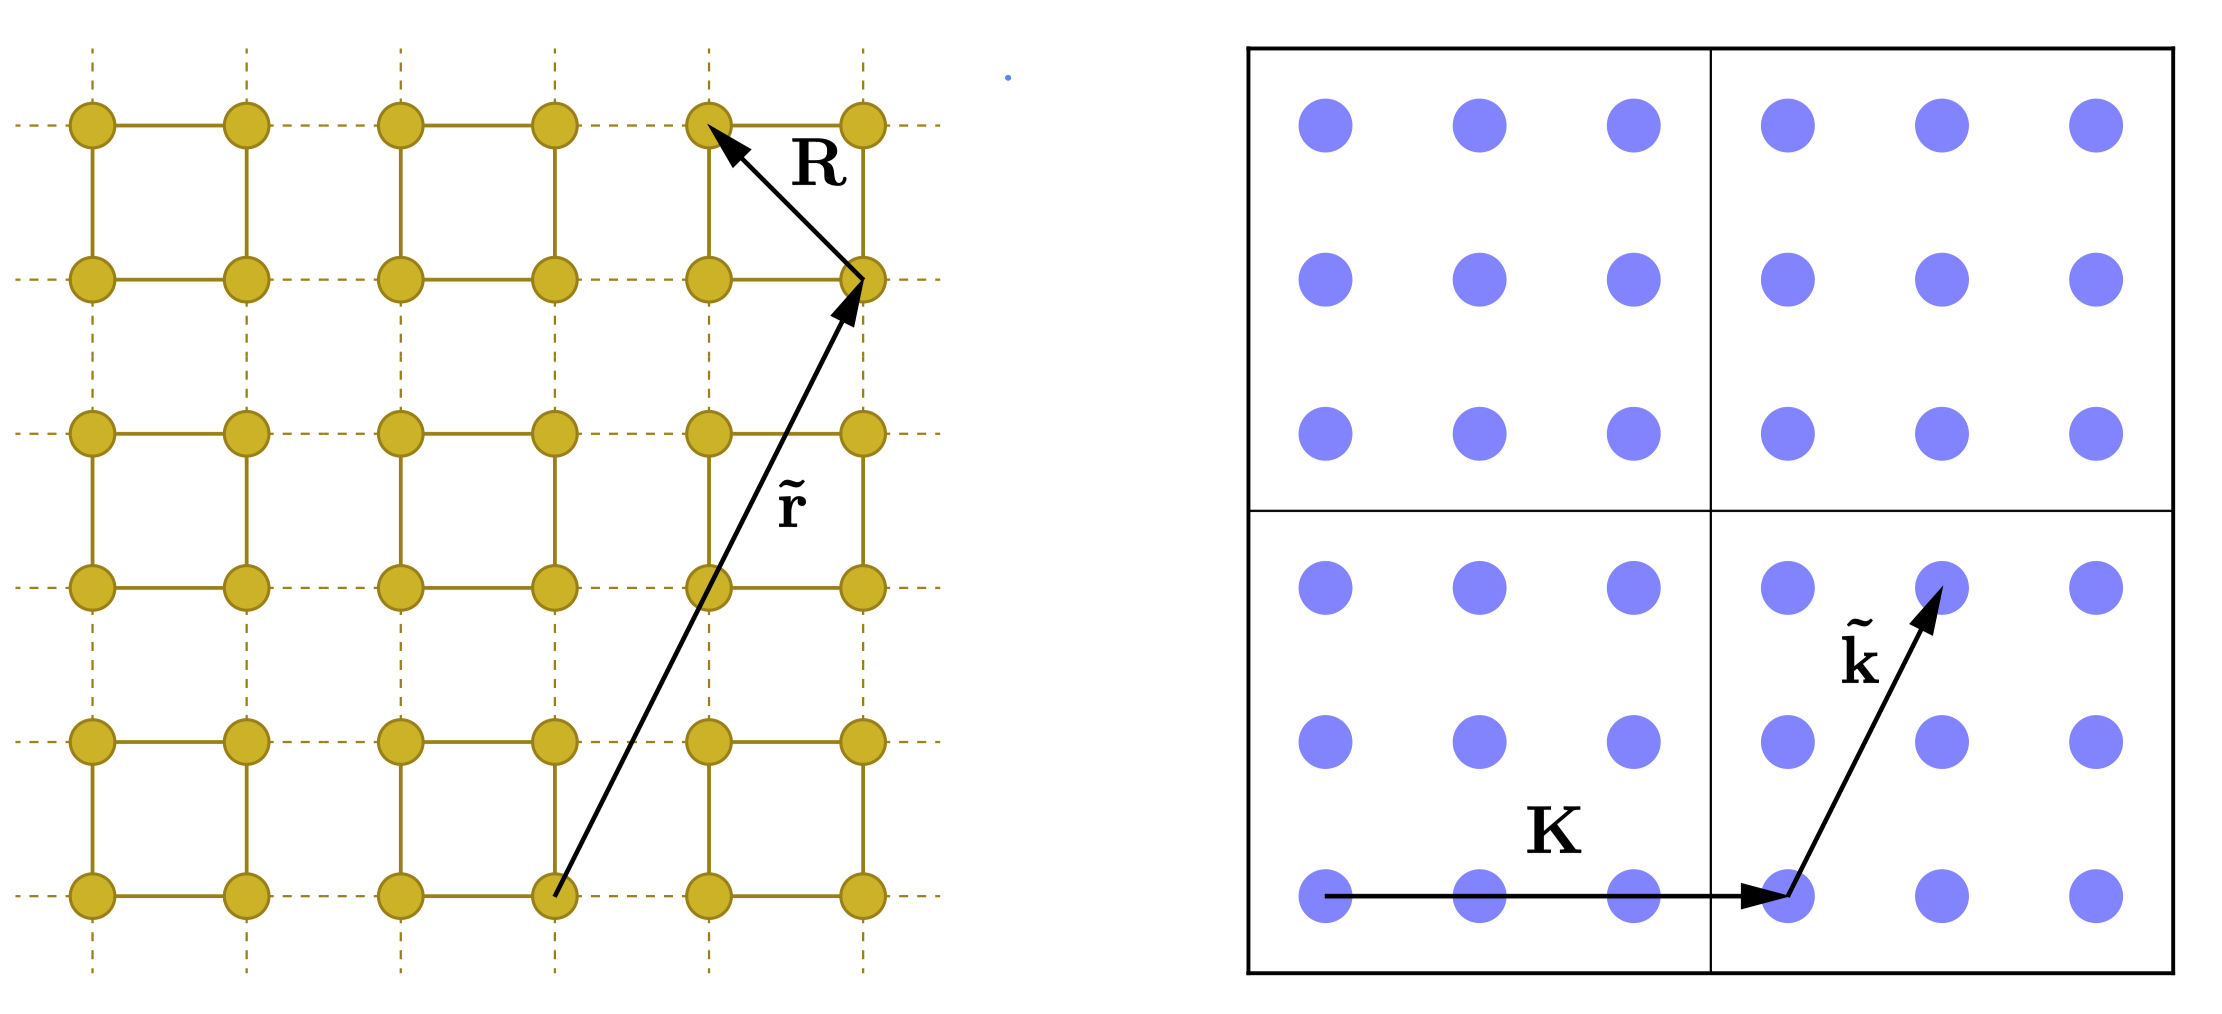
\includegraphics[scale=0.25]{./figures/theory/mixed_basis.png}
    \end{figure}
    \footnotetext{Maxime Charlebois. "Théorie de champ moyen dynamique pour les
    système inhomogènes". \textcolor{hard_green}{Thèse de doct. Université Laval 2015}.}
\end{frame}

\begin{frame}
    \frametitle{Théorie - Formalisme de Green}
    Grâce à ce choix de base, on sépare les dépendances inter-intra amas comme
    \begin{align*}
        \vb{\Sigma} = \vb{\Sigma}_c(\vb{R}, z) + \vb{\Sigma}(\vb{\tilde{k}}, z),
        &&\vb{t} = \vb{t}_c(\vb{R}) + \vb{t}(\vb{\tilde{k}})
    \end{align*}
    \vfill
    \pause
    en ayant utilisé les transformées de Fourier partielles suivantes
    \begin{align}
      f(\vb{R}, \vb{\Tilde{r}}) &= \frac{N_c}{N}\sum_{\vb{\Tilde{k}}}e^{i\vb{\Tilde{k}}\cdot\vb{\Tilde{r}}}f(\vb{R}, \vb{\Tilde{k}})\\
      f(\vb{R}, \vb{\Tilde{k}}) &= \sum_{\vb{\Tilde{r}}}e^{-i\vb{\Tilde{k}}\cdot\vb{\Tilde{r}}}f(\vb{R}, \vb{\Tilde{r}}),
      \label{eq: partial_fourier}
    \end{align}
\end{frame}
